\begin{figure}[ht!]
\centering
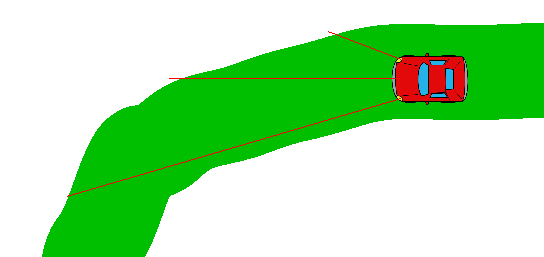
\includegraphics[width=65mm]{data/car1.png}
\caption{Els sensors detecten la distància del cotxe a les parets del circuit.}
\label{sensors}
\end{figure}

La nostra segona demostració és radicalment diferent a la primera:
l'objectiu és programar un automòbil el qual, a partir de tres sensors frontals,
sigui capaç de evitar xocar amb les parets de \emph{qualsevol circuit}.
És a dir; el seu entrenament ha de ser general i adaptable a qualsevol situació.

Per a solucionar un problema com aquest, no disposem d'un \emph{dataset},
com en el cas del reconeixement de caràcters: qui s'ha dedicat a crear
una base de dades que representa totes les decisions que hauria de prendre
el cotxe, en qualsevol dels casos en que es pot trobar? Evidentment, no és
una tàctica adequada.

Hem d'atacar el problema des d'un altre punt de vista: ara ja no es tracta
d'una situació en la qual l'entrenament de l'agent es pugui supervisar
(\emph{supervised learning}), ara ha d'ésser l'agent qui explori l'entorn
en el qual es troba.
